\documentclass[../report.tex]{subfiles}
\def\code#1{\texttt{#1}}
\begin{document}
\onehalfspacing

\section{Appendix}

The code for this report is based off of Google's Verified Boot reference repository\cite{vboot-codebase} and the modifications can be accessed in a cloned and edited repository\cite{my-repo}.
Changes were restricted to the created folder \code{tests/cbmc} within the repository.
In order to minimize changes to the existing codebase, if functions were edited elsewhere, these changes would only take effect if the C macro ``\code{CBMC}'' is defined. 

\subsection{Images} 
\begin{figure}
  \centering
  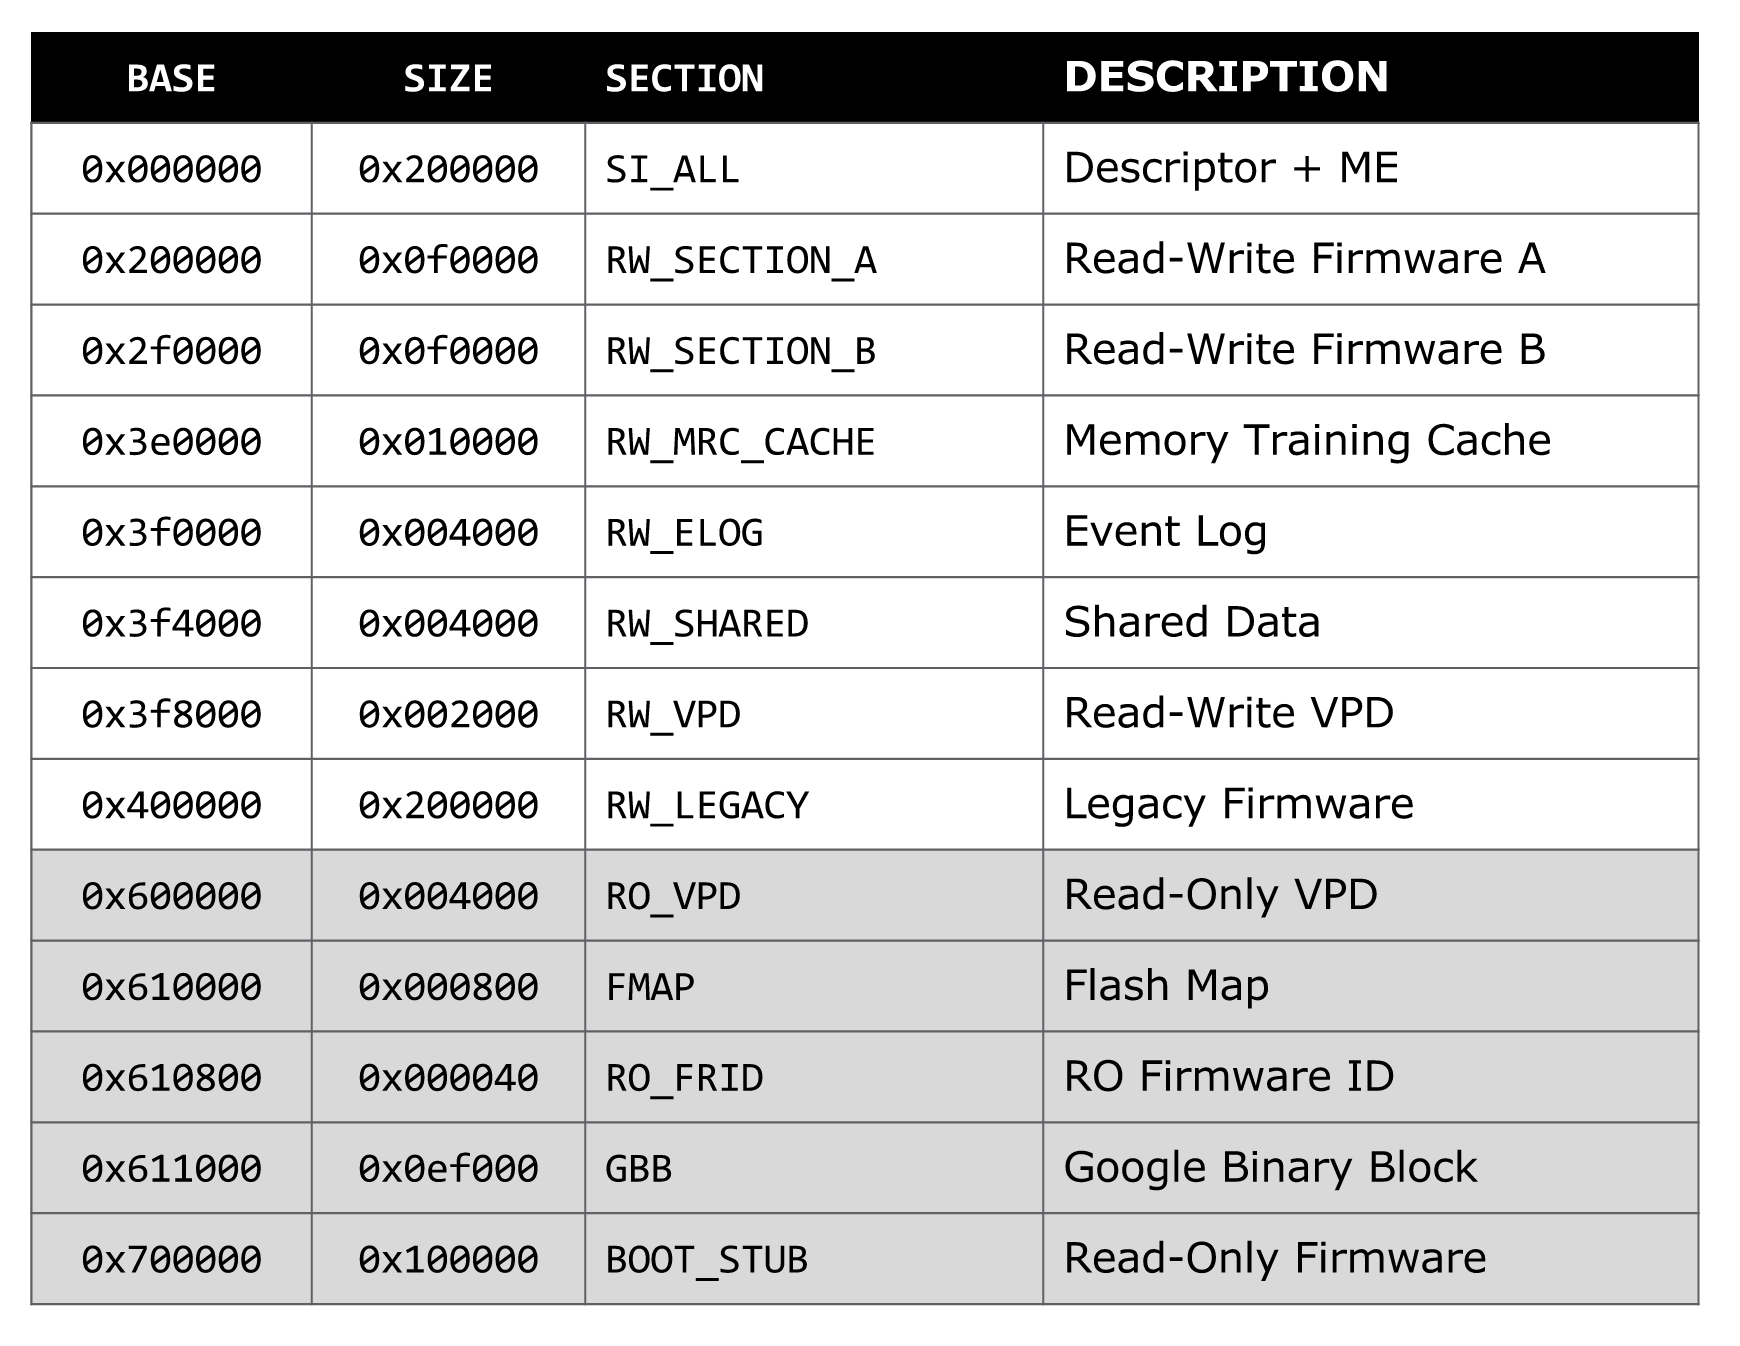
\includegraphics[width=0.8\linewidth]{fmap_locs.png}
  \caption{The Flash Map for Chrome OS's SPI Flash. The gray sections have been marked as Read Only~\cite{fw-summit}}
  \label{fig:fmap}
\end{figure}

\subsection{CBMC Commands}

Python scripts have been created to generate the CBMC command for different C files.
These scripts are based off of a simple base script with the following editable arrays.

\begin{itemize}
    \item \code{includedDirs}  --- list of all directories with related C header files 
    \item \code{includedFiles} --- list of all C file with necessary functions
    \item \code{extras} --- list of CMBC specific commands including array bounds checking, C Macro definitions, and loop unwinding limits 
\end{itemize}

\subsection{CBMC Output}

The most helpful function of CBMC is its ability to provide a trace of variables that provides a counterexample to a given assertion. 
However, the size of the codebase and the number of possible set variables makes it difficult to manually examine the counterexample to see what exactly is causing the assertion to be proved incorrect.
For this reason I have created the \code{parse\_output.py} file which takes in CBMC output and displays the non-deterministic variables in a formatted manner. 
The most helpful aspect of this program is that it is able to parse the binary flags and reveal in human readable format what is enabled or disabled.

% \subsection{Full Runthrough}

% \subsection{Vagrant}


% \begin{table*}\centering
%     \caption{Configurable Arrays within CBMC command framework}\label{sfw_results}
%     \begin{tabular}{p{0.3\linewidth}p{0.6\linewidth}}\toprule
%     \arraystretch{2}
%         Array Name & Description \\ \bottomrule 
%         includedDirs  & list of all directories with related C header files \\ 
%         includedFiles & list of all C file with necessary functions \\
%         extras & list of CMBC specific commands including array bounds checking, C Macro definitions, and loop unwinding limits \\ 
%         \bottomrule
%     \end{tabular}
% \end{table*}

\end{document}
